\documentclass{article}
\usepackage[top=2cm, bottom=2cm, left=2cm, right=2cm]{geometry}
\usepackage{graphicx}
\pagestyle{empty}
\begin{document}
\section*{2016 olympiad not-swaps}

\vfill\vfill\vfill

\includegraphics[scale=2]{data/pix/swaps11.eps}\vfill\vfill

\includegraphics[scale=2]{data/pix/swaps13.eps}\vfill\vfill\vfill~
\newpage
\section*{1st moves: E13-dot, E15-black, D15-white, M15-blackwhite}
\vfill

{\large\bf MoHex loss 11x11 D-M 1.g2 2.swap 3.e4 \ldots}
\vfill\vfill

\includegraphics[scale=2]{data/pix/1stmove11.eps}\vfill\vfill

{\large\bf MoHex loss 13x13 D-M 1.j2 2.g8 3.d10 \ldots}

{\large\bf MoHex loss 13x13 D-M 1.d2 2.e9 3.g8 \ldots}
\vfill

\includegraphics[scale=2]{data/pix/1stmove13.eps}\vfill\vfill\vfill~
\newpage
\section*{mohexnet-v-mohex results: opening a1\ldots\ a13}
\begin{figure}[hb]
\includegraphics[scale=2]{data/pix2/mnt-mx.eps}\vfill\vfill\vfill~
\caption{Mohexnet win rates by first move and color. Opening moves: a1\ldots a13. Black plays first. 
Column a: 3s, min ?, rel1000.
Column b: 3s, min ?, rel2000. 
Column c: mohex-mohex. 
Column d:3s, min 100, rel1000.
Column e:3s, min 10, rel1000. 
Column f:3s, min 40, rel1000.
Column g:3s, best. ~ ~ ~ ~ 
Column l:3s, best.
Column m: mohex-mohex.}
\end{figure}
\end{document}
